\newpage
\section{Struttura}

\epigraph{Direzioni cristallografiche |u v w| dove sono numeri interi, è come un vettore normale i cui vettori di base sono quelli primitivi}{\textit{Leonardo Sabattini}, I edizione}

Possiamo raggruppare i solidi in tre gruppi principali:
\begin{itemize}
    \item Cristallini.
    \item Amorfi.
    \item Parzialmente cristallini.
\end{itemize}
Le strutture ordinate si ottengono grazie alle interazioni elettrostatiche che si creano (legami covalenti, metallici, interazioni dipolo-dipolo). Al di sotto di una certa temperatura queste interazioni vincono i moti termici e, nel caso di atomi, questi si organizzano in un \textbf{\textit{reticolo cristallino}}, strutture periodiche ordinate definite da 3 vettori \textbf{\textit{primitivi}} a partire dai quali è possibile generare tutto il reticolo. In generale in ogni punto del reticolo possono trovarsi uno o più atomi; poiché non è sempre possibile individuare tutti i punti del reticolo partendo da un solo punto del reticolo in alcune strutture è necessario definire una base costituita da più punti; il caso più semplice sono i monocristalli.
L'organizzazione spaziale degli atomi in 3D rispetta uno dei 14 reticoli di Bravais (230 gruppi spaziali se si aggiungono anche le simmetrie). Non tutti reticoli cristallini hanno la stessa efficienza nell'impacchettare gli atomi: più compatti sono l'FCC (face centered cubic) ed l'HCP (Hexagonal close packed), entrambi hanno un atomic packing factor di 0,74 (entrambi sono ottenuti allo stesso modo ma posizionando le sfere in maniera sfalsata). Sapere la struttura cristallina è molto importante in quanto molte proprietà dei materiali dipendono da essa.
Definiamo alcune cose che possono essere utili:
\begin{itemize}
    \item Direzioni cristallografiche |u v w| dove sono numeri interi, è come un vettore normale i cui vettori di base sono quelli primitivi; con <u v w> si indica una famiglia (sono caratterizzati dalla stessa distanza atomica: |1 0 0|, |0 1 0|, ...).
    \item Piani cristallini (h k l), le lettere indicano le celle in cui il piano si interseca; una famiglia di piani è definita come \{ h k l \} (piani distanziati ma paralleli).
\end{itemize}
In generale è importante sapere quali piani cristallini e quali direzioni presentano la massima densità in quanto alcuni processi dipendono da esso. Un'altra cosa importante che è associata alla struttura cristallina sono i suoi \textbf{\textit{siti interstiziali}}. Sono importanti in quanto artefici della diffusione di altre specie all'interno di un materiale. Il rapporto tra i raggi della specie che si vuole aggiungere al cristallo e quello già presente determina il tipo di interstizio ed il numero di coordinazione della specie: se il rapporto è piccolo si occuperà una cavità tetraedrico, all'aumentare delle dimensioni si avrà coordinazione ottaedrica e, per raggi molto simili, anche strutture cubiche.\\
In generale non si ha mai un cristallo unico ma si lavora con un materiale policristallino, formato cioè da molti cristalli più piccoli detti \textbf{\textit{grani}}, sono separati tra loro da \textbf{\textit{bordi di grano}}. In generale però si possono avere anche strutture non ordinate, ad esempio quando il raffreddamento dalla fase liquida è talmente veloce da bloccare la diffusione ed impedire la riorganizzazione in un reticolo cristallino. Si ottiene allora un sistema metastabile e tendenzialmente una struttura amorfa. Alcuni polimeri possono raggiungere un grado di cristallinità elevato mantenendo comunque un certo grado di disordine.

    \begin{figure}[h]
    \centering
  \begin{minipage}[b]{0.3\linewidth}
    \centering
    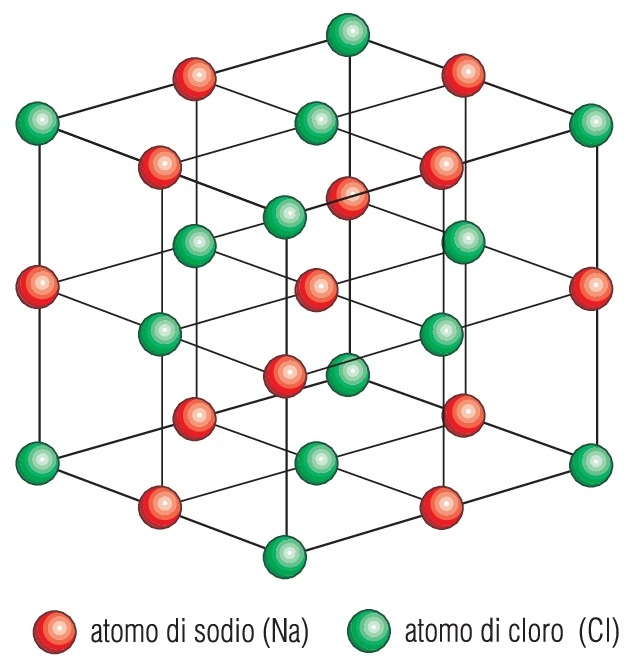
\includegraphics[width=\linewidth]{struttura/cristallo.jpg}
    \label{cristallo}
  \end{minipage}
  \begin{minipage}[b]{0.3\linewidth}
    \centering
    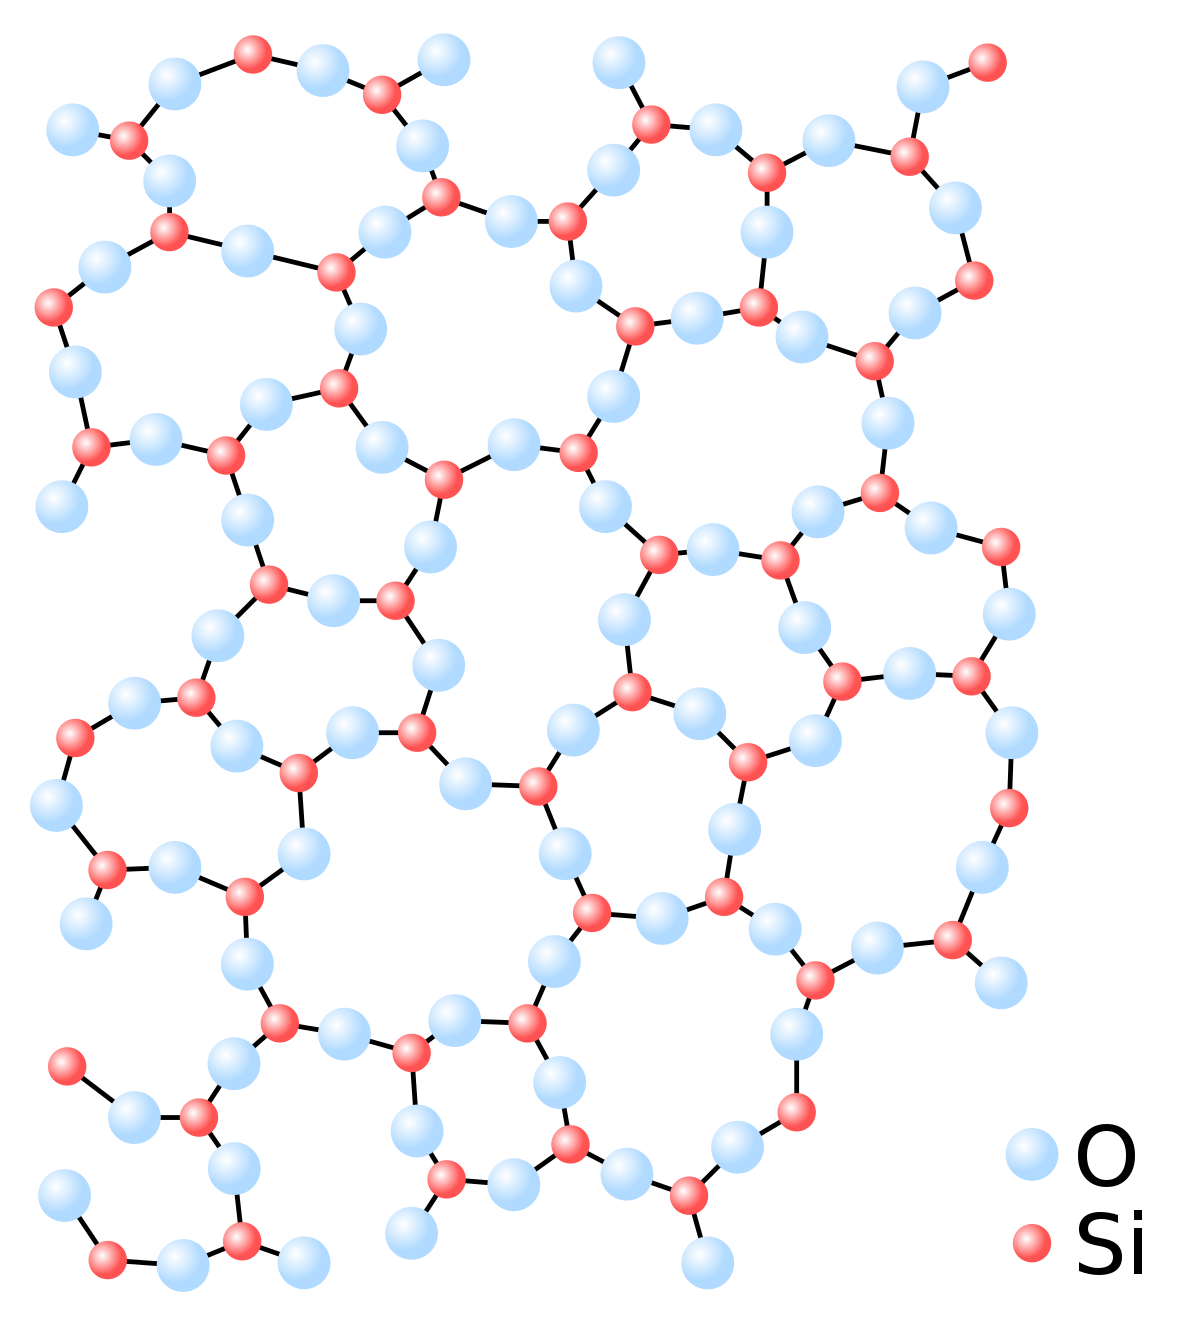
\includegraphics[width=\linewidth]{struttura/amorfo.png}
    \label{amorfo}  

  \end{minipage}
    \begin{minipage}[b]{0.3\linewidth}
    \centering
    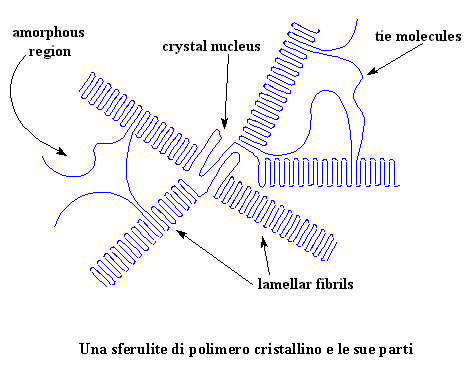
\includegraphics[width=\linewidth]{struttura/polimero,semicristallino.jpg}
    \label{semi}  

  \end{minipage}

  \caption{Sinistra: cristallo, struttura amorfa, struttura semicristallina.}
  
\end{figure}

\subsection{Solidificazione dei metalli}
La solidificazione avviene ovviamente per motivi termodinamici ovvero quando l'energia libera della forma solida è uguale a quella della fase liquida. In generale la pendenza (rappresentata dall'entropia) della fase liquida è maggiore di quella della fase solida, e quindi a T più alta la prima risulta più stabile.
All'equilibrio si ha:
\begin{equation}
    \Delta G_V=G_s-G_v=0
\end{equation}
Se la temperatura diminuisce la fase solida diventa più favorita ed il contributo è sempre negativo; bisogna però considerare bene questo processo in si crea un'interfaccia tra le due fase. Una descrizione quantitativa di questo fenomeno richiede l'introduzione della tensione superficiale:
\begin{equation}
    \Delta G_T=\frac{4}{3}\pi r^3\Delta G_V+\gamma\pi r^2
\end{equation}
dove $\gamma$ è la tensione superficiale ed è sempre positiva. La nucleazione e l'eventuale formazione di cristalli possono avvenire solo se si riesce a superare una certa dimensione critica:
\begin{equation}
    r^*=-\frac{2\gamma}{\Delta G_v}=-\frac{2\gamma T_m}{\Delta H_v(T_m-T)}
\end{equation} 
Questa dimensione deve essere la minore possibile in quanto l'energia massima del processo dipende da questa quantità (anche $\gamma$ dovrebbe essere una funzione di T in realtà).
Il valore del raggio critico definisce il rate di creazione di questi cristalli:
\begin{equation}
    v_d=K_1\exp(-\frac{\Delta G*}{kT}
\end{equation}
Un altro processo che entra in gioco è la diffusione:
\begin{equation}
    v_d=K_2\exp\left(-\frac{Q_d}{KT}\right)
\end{equation}
Questo processo di cristallizzazione è detto \textbf{\textit{omogenea}}.
Spesso la cristallizzazione avviene però in maniera \textbf{\textit{eterogenea}}, sfruttando cioè la presenza di superfici o di cristalli già esistenti; in questo caso è più facile ottenere un raggio di curvatura maggiore del raggio critico. Inoltre, questo metodo richiede temperature di sottoraffreddamento minori.

\subsection{Microstrutture}

\epigraph{sono i primi a formarsi a causa delle superfici fredde della forma}{\textit{Leonardo Sabattini}, I edizione}

La struttura di grano dipende molto da come il materiale è stato raffreddato ed è importante per capire le proprietà meccaniche di un oggetto. Materiali che presentano strutture di grano sottili sono in genere più resistenti a temperature basse, mentre il comportamento si inverte quando si lavora ad alte temperature, ed è quindi preferito lavorare con monocristalli.
\begin{figure}[h]
    \centering
    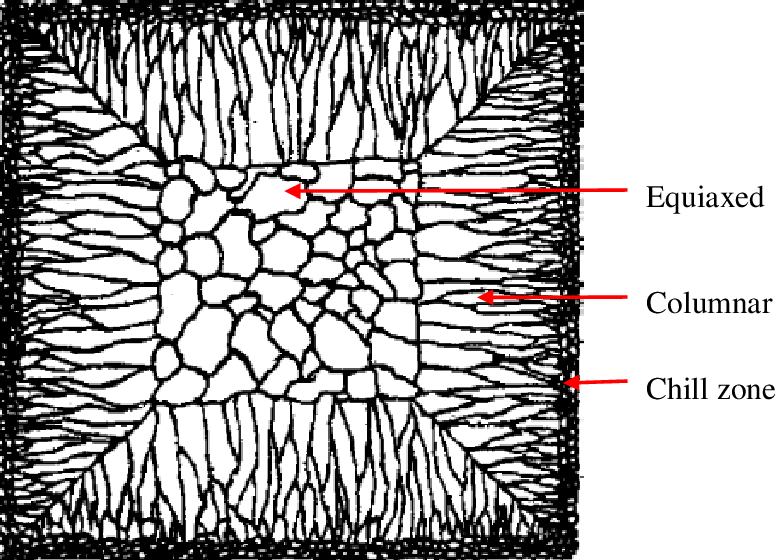
\includegraphics[width=6cm]{struttura/colata_grain.png}
    \caption{Struttura di grano.}
    \label{colata}
\end{figure}
In generale durante la colata si generano grani di dimensione differente (rappresentati in Fig \ref{colata}):
\begin{itemize}
    \item Chill zone: sono i primi a formarsi e si trovano lungo la superficie dello stampo, nella regione che si raffredda per prima. \textcolor{red}{DA RICONTROLLARE hanno dimensioni piccole e forma irregolare; da loro dipende la durezza del manufatto}
    \item Columnar zone: la forma di questi grani è associata ai moti convettivi e al modo in cui il calore fluisce dal centro del campione verso l'esterno, pertanto sono allungati ed ortogonali alle pareti dello stampo.
    \item Equiaxial zone: hanno nuovamente una dimensione piccola, sono dovuti alla presenza di elementi di lega od in generale alla presenza di altre specie come raffinatori di grano, di solito hanno una forma tonda ed un orientazione randomica.
\end{itemize}
Per ottenere grani più piccoli vengono usati i cosiddetti \textbf{\textit{raffinatori di grano}}. La colata su di una forma non è l'unico modo di lavorazione, altri metodi procedono per colata continua (ad esempio quelli utilizzati per la produzione dell'acciaio).
Se vogliamo ottenere invece monocristalli è necessario ricorrere ad altre tecniche specifiche; ad esempio si può usare il processo "pigtail" in cui si usa uno strumento a forma di coda di maiale che permette l'eliminazione e la crescita selettiva di cristalli con una particolare orientazione (questo metodo è impiegato per produrre turbine monocristalline che lavorano ad alta T). Un altro metodo visto a lezione sfrutta un singolo cristallo già esistente che funge da seme, permettendone l'accrescimento tramite opportuna modulazione della temperatura e delle condizioni di lavoro. Affinché il processo venga bene, infatti, il liquido in contatto con il cristallo deve essere ad una temperatura molto vicina a quella di fusione instaurando un equilibrio (con questo metodo viene sintetizzato il silicio monocristallino). Ovviamente i metodi usati per produrre materiali monocristallini sono generalmente più costosi degli altri.

\section{Imperfezioni}

\epigraph{I due tipi più sono: a vite o a spigolo o miste.}{\textit{Leonardo Sabattini}, I edizione}

Ci sono diversi tipi tipi di imperfezioni nei cristalli con una conseguente perdita di periodicità. Non tutti i difetti sono accidentali, spesso si aggiungono di proposito come accade col drogaggio dei semiconduttori.
Le imperfezioni sono classificate in base alla dimensionalità:
\begin{itemize}
    \item \textbf{\textit{Difetti puntuali (0D)}}: sono di vario tipo: interstiziali, quando si ha una specie estranea all'interno degli spazi vuoti del reticolo, oppure sostituzionali, quando la specie è sostituita con un altro elemento. 
    Un altro tipo di imperfezioni sono rappresentate dalle vacanze, ovvero posizioni cristalline in cui si ha l'assenza di un atomo; questo può essere dovuto ad esempio a vari processi durante il processo di raffreddamento. 
    Questi difetti creano delle tensioni che coinvolgono le immediate vicinanze ma che tendono a scomparire a grandi distanze.
    In aggiunta, nei solidi ionici abbiamo:
    \begin{enumerate}
        \item Difetti di Frenkel, dove uno ione è spostato dalla sua posizione nel reticolo e occupa una posizione interstiziale.
        \item Difetti di Schottky, dove si ha una vacanza sia di un catione che di un anione (per preservare l'elettroneutralità).
    \end{enumerate}
    L'origine dei difetti puntuali (mostrati in fig. \ref{defects}) può essere di varia natura, ad esempio potrebbe essere dovuto al processo di raffreddamento troppo veloce che non permette il raggiungimento dell'equilibrio, in ogni caso la loro presenza comporta sicuramente un aumento dell'entropia. La frazione di siti difettati (Shottky o Frenkel) può essere stimato usando la legge di Boltzmann:
    \begin{equation}
        \chi_{dif}=\exp\left(-\frac{E_{dif}}{KT}\right)
    \end{equation}
    La legge scritta sopra è valida solo in condizioni di equilibrio.
    \begin{figure}[h]
        \centering
        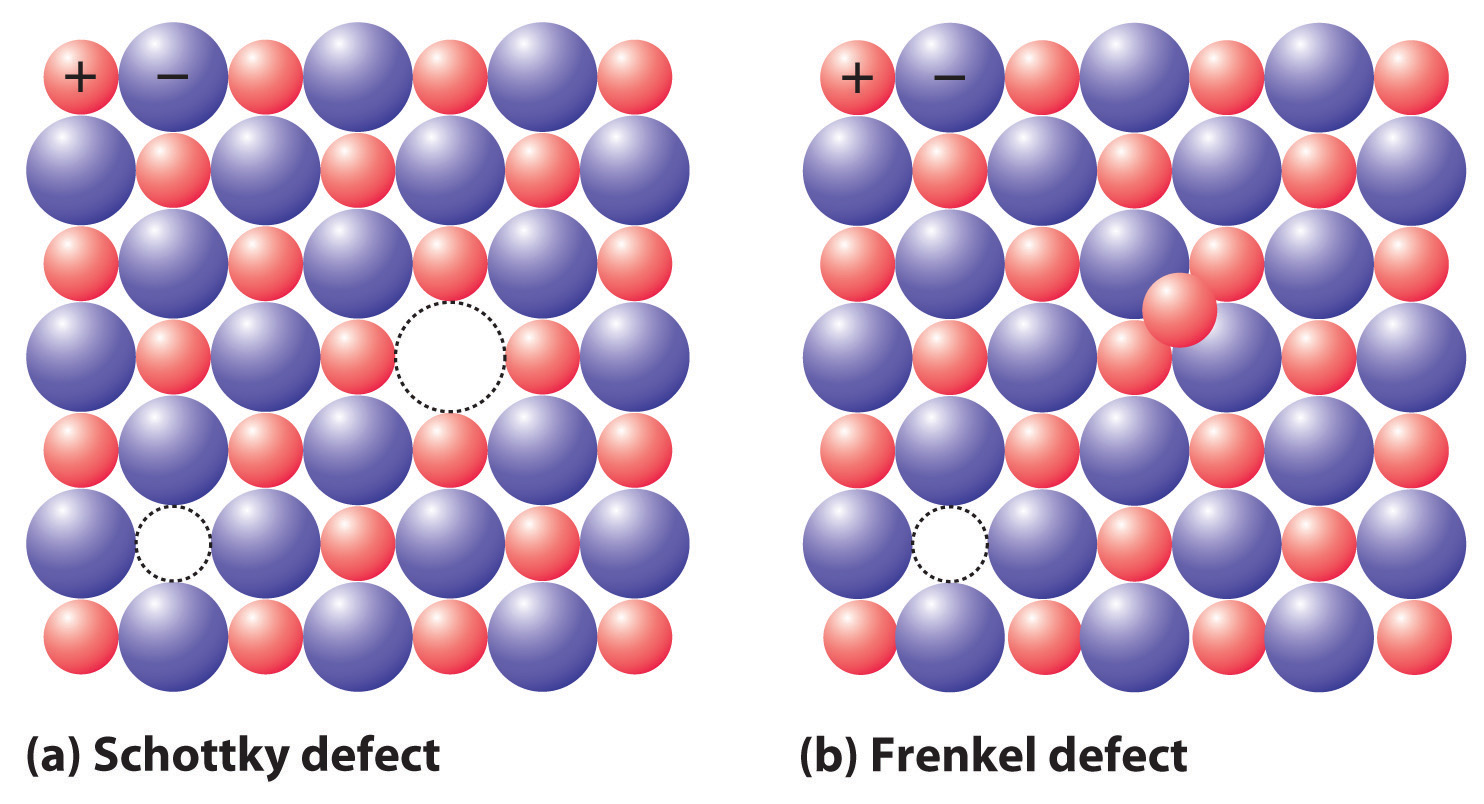
\includegraphics[width=5cm]{struttura/shottky.jpg}
        \caption{Tipi di dislocazioni puntuali: sinistra è di tipo Shottky, destra è di tipo Frenkel.}
        \label{defects}
    \end{figure}
    \item \textbf{\textit{Difetti 1D}}: vengono anche chiamate dislocazioni, e sono determinanti in molti processi e fenomeni che determinano le proprietà meccaniche dei materiali, soprattutto la plasticità. I due tipi di dislocazioni che individuiamo sono quelle a vite e quelle a spigolo; esistono anche le dislocazioni miste che sono una combinazione delle due tipologie precedenti. Possono essere dovute a deformazioni plastiche che inducono lo spostamento di filari di atomi, ma anche a raggruppamento di vacanze. La natura della dislocazione viene definita dal vettore di Burgers: la direzione è perpendicolare alla dislocazione mentre il modulo è uguale alla distanza rispetto alla posizione di equilibrio.
        \begin{figure}[h]
    \centering
  \begin{minipage}[b]{0.4\linewidth}
    \centering
    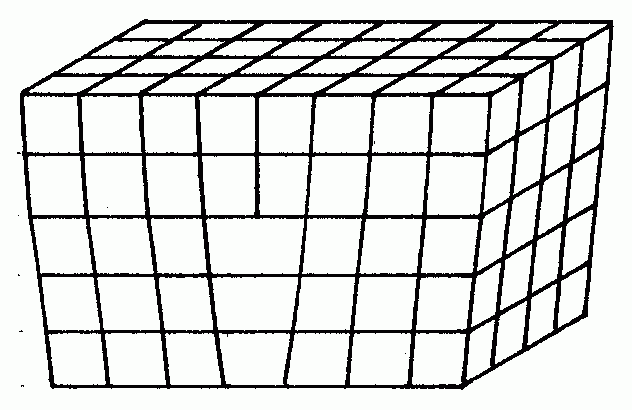
\includegraphics[width=\linewidth]{struttura/screw_dislo.png}
    \label{screw}
  \end{minipage}
  \begin{minipage}[b]{0.4\linewidth}
    \centering
    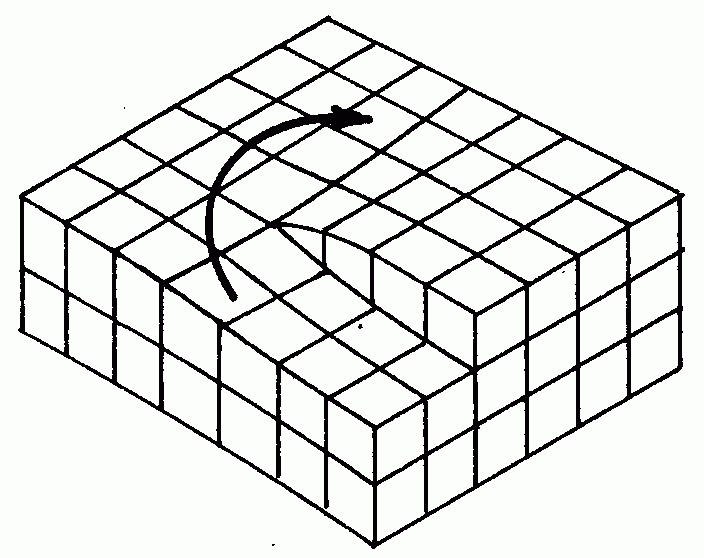
\includegraphics[width=\linewidth]{struttura/Dislocation_hélicoïdale.png}
    \label{dislo}  

  \end{minipage}
  \caption{Sinistra: dislocazione a spigolo, destra: a vite}
\end{figure}
    \item \textbf{\textit{Difetti di superficie}}: i difetti di superficie più frequentemente incontrati sono i bordi di grano. Nei bordi di grano si raggruppano le imperfezioni e spesso agiscono come centri di nucleazione. Altri difetti bidimensionali sono gli stacking e il twinning. I bordi di grano sono zone in cui due monocristalli, generalmente con orientazione differente, si incontrano, e tipicamente hanno uno spessore pari a qualche passo reticolare.
    \item \textbf{\textit{Difetti di volume}}: lo si ha quando diversi difetti puntuali si raggruppano.
\end{itemize}

\subsection{Diffusione nei solidi}

\epigraph{Deformazioni plastiche+come avvengono deformazioni e come sono involuite le dislocazioni}{Sun Tzu, \textit{l'arte della guerra [contro la lingua italiana, ndr]}}

Il processo di diffusione avviene tanto nei liquidi quanto nei solidi. Affinché la diffusione avvenga è necessario superare un'energia di attivazionem in quanto essa segue una cinetica di tipo Arrhenius. 
La diffusione si ha principalmente nei solidi con difetti sostituzionali e interstiziali. La velocità di diffusione dipende dall'energia che a sua volta dipende dalla natura dal reticolo cristallino e dalla natura della specie che diffonde: si osserva che nei solidi con difetti interstiziali è più bassa rispetto a quelli sostituzionali; per dare ordini di grandezza, se le prime sono sui 10 kcal/mol, le seconde stanno sopra i 50 kcal/mol.
Alcuni esempi che utilizzano la diffusione nei solidi sono la precipitazione di solidi (la creazione di leghe), il moto dei difetti e la nucleazione di nuovi grani. 

La diffusione allo stato stazionario segue la legge di Fick:
\begin{equation}
    J(x)=-D\frac{\partial C(x)}{\partial x}
\end{equation}
Dove $J$ è il flusso su una superficie e $D$ è la diffusività [m/s$^2$]. D dipende da tanti fattori:
\begin{itemize}
    \item Dalla struttura cristallina.
    \item Dalla temperatura.
    \item Dalla concentrazione di soluto.
    \item Dalla presenza di difetti.
\end{itemize}.
In condizioni non stazionarie si segue invece la seconda legge di Fick:
\begin{equation}
    \frac{\partial C(x,t)}{\partial t}=\frac{\partial }{\partial x}\left(-D\frac{\partial C(x)}{\partial x}\right)
\end{equation}
Sapere come si comporta la diffusione è importante in quanto diversi processi industriali ne fanno utilizzo come la carburazione dell'acciaio, il doping dei semiconduttori e la sinterizzazione delle ceramiche. Nei materiali ceramici dove sono presenti legami ionici la situazione è più complessa, in quanto l'elettroneutralità va conservata e quindi i processi diffusivi di specie cariche coinvolgono sempre almeno due specie differenti, limitando la diffusione alla specie più lenta.
Le deformazioni avvengono nei piani con la maggiore densità atomica e lungo le direzioni con la maggiore densità lineare.
Nei cristalli ionici le cose sono più complicate in quanto fatto da ioni di carica opposta: lo scorrimento può avvenire lungo la direzione che non implica la sovrapposizione di atomi con lo stesso segno.
Twinning and shear force (avviene meglio per HCP: struttura rombica, sensato). 

\subsection{Meccanismi d'indurimento e rafforzamento}

Esistono diversi metodi di rafforzare un manufatto. In generale si cerca di agire su difetti e dislocazioni in modo da ostacolarne la propagazione e quindi aumentare la rigidezza del campione; un'altra soluzione, impraticabile il più delle volte, consiste nel creare monocristalli perfetti.

\begin{itemize}
    \item Creazione di soluzioni solide
    \item precipitazioni di nanofasi
    \item Rafforzamento dei bordi di grano
    \item Incrudimento.
\end{itemize}

\subsection{Soluzioni solide e precipitazione di nanofasi}

I metalli puri presentano piccoli valori di snervamento, per questo viene aggiunto un secondo elemento (nelle soluzioni solide) o una seconda fase per migliorarne le proprietà meccaniche.
Nelle soluzioni solide viene sostituito parzialmente il nostro elemento con un'altra specie con dimensioni differenti che andranno ad aumentare il numero di dislocazioni aumentandone la rigidezza senza però modificare in maniera sostanziale altre proprietà.
Nell'incrudimento per precipitazione invece si crea proprio una nuova fase che andrà a limitare ancora di più il movimento delle dislocazioni. Più queste nanofasi saranno piccole e finemente disperse maggiore sarà l'ostacolo.
Nelle \textbf{\textit{leghe di metalliche}} si crea un miscuglio omogeneo tra il nostro elemento iniziale che funge da solvente ed elementi esterni, chiamati elementi di lega, che fungono da soluti. In generale possiamo avere  \textbf{\textit{substitutional solid solutions}} or  \textbf{\textit{interstitial solid solutions}}.
Le leghe metalliche di solito hanno proprietà simili al metallo iniziale con la differenza che le T$_m$ non è più precisa ma spesso è un intervallo; si parla quindi di \textbf{\textit{fusione incongruente}}.
Le soluzioni solide possono essere di più tipi:
\begin{itemize}
    \item  \textbf{\textit{primario}} se la struttura cristallina viene mantenuta.
    \item  \textbf{\textit{secondario}} se la struttura cristallina della lega è differente da quella del metallo più abbondante (si verifica raramente).
    \item  \textbf{\textit{composti intermetallici}} se è un composto chimico vero e proprio con delle proporzioni precise. In questo caso non si ha più il tipico legame metallico ma spesso ha forte carattere covalente ed emergono proprietà differenti dai metalli soliti.
\end{itemize}
Perchè si formi una \textbf{\textit{soluzione solida sostituzionale}}(l'elemento di lega si va a sostituire al nostro elemento nel reticolo) empiricamente si è osservato che:
\begin{enumerate}
    \item I due elementi devono presentare dimensioni simili (raggio atomico differente al più del 15\%).
    \item Avere stesso reticolo cristallino.
    \item Avere simile elettronegatività.
    \item Avere stessa valenza.
\end{enumerate}
Queste regole sono dette regole di \textbf{\textit{Hume-Rothery}}. In caso di solubilità parziale empiricamente si osserva che l'elemento che ha maggiore valenza presenta una maggiore solubilità.
Per ottenere una \textbf{\textit{soluzione solida interstiziale}}, invece, le dimensioni del soluto devono essere minori di quelle del solvente e rispettare rapporti abbastanza stringenti; di solito solo O, B, H, C, N riescono a dare questo tipo di soluzioni.
In genere le soluzioni solide mantengono le proprietà metalliche diventando però più dure e resistenti a causa delle tensioni interne; le proprietà di trasporto però peggiorano.
La dimensione dell'elemento di lega influisce sulla tensione che genera alla struttura e quindi anche all'impatto che esso provoca al campione. Una piccola aggiunta di berillio aumenta molto la tensione di snervamento del rame rispetto allo zinco o al nichel che presentano dimensioni simili.

\subsection{Precipitation hardening}

La precipitazione avviene quando la variazione di energia libera è negativa:
\begin{equation}
    \Delta G_T=(\Delta G_{\alpha\rightarrow\beta}+\epsilon)\frac{4\pi r^3}{3}+4\pi \gamma r^2
\end{equation}
$\epsilon$ rappresenta l'energia di strain che si genera a causa della riorganizzazione che avviene all'interno del reticolo. Se si hanno \textbf{\textit{precipitati coerenti}}, ovvero se i reticoli delle due fasi si sovrappongono bene, il termine di strain è minimo. La precipitazione avviene in due step:
\begin{itemize}
    \item Nucleazione: avviene nelle zone dove il termine di strain e di tensione superficiale hanno minor impatto, ovvero nei bordi di grano 
    \item Crescita: la crescita avviene principalmente attraverso la diffusione di atomi e quando i costituenti sono molto legati al reticolo ne rappresenta il principale impedimento.
\end{itemize}
Perché avvengano precipitation hardening o age hardening occorre che:
\begin{itemize}
    \item La solubilità della lega deve diminuire al diminuire di T. 
    \item La lega deve presentare una singola fase ad alta T e separarsi in due fasi per temperature opportune.
    \item La matrice deve essere duttile e non dura mentre il precipitato deve essere un composto intermetallico fragile e duro.
    \item La lega deve essere estinguibile (quenchable), cioè deve permettere al campione di raffreddarsi dalla fase unica ad alta temperatura senza che si separi in due fasi distinte.  
    \item Il precipitato deve essere coerente.
\end{itemize}
L'age hardening avviene per tre step:
\begin{enumerate}
    \item Solution Treatment: Si scalda la soluzione a T$>$T$_{solvus}$ in modo da ottenere una singola fase.
    \item Quench: Si raffredda il materiale non dando il tempo al materiale di separare le fasi ed ottenendo una fase metastabile con il soluto.
    \item Aging: il sistema soprasaturo viene mantenuto a T$_{amb}$ (natural aging) o riscaldato a T inferiore di T$_{solvus}$ (artificial). La temperatura e il tempo di esposizione modificheranno la dimensione dei grani e quindi la resistenza del nostro campione. Se il tempo di esposizione è poco si avranno precipitati piccoli e poco sviluppati, se si aspetta troppo avremo precipitati troppo accresciuti e si raggiunge nuovamente l'equilibrio, quello che avremmo ottenuto raffreddando lentamente il campione.
\end{enumerate}

\subsection{Grain Boundary strenghtening \& cold workinng}

La dimensione dei grani influisce sulla resistenza del nostro materiale.
Più la grana è fine maggiore sarà la tensione di snervamento. Si ha una legge empirica delle \textbf{\textit{Hall-Petch equation}} che dice:
\begin{equation}
    \sigma_y=\sigma_0+\frac{K_y}{\sqrt{d}}
\end{equation}
Dove $K$ e $\sigma_0$ sono costanti tipiche del materiale. Questa legge non vale sempre: se $d$ diventa troppo piccolo il materiale viene considerato amorfo e non possono più essere definite le dislocazioni. Il massimo si ha intorno a 10-15nm; al di sotto di queste dimensioni il meccanismo della deformazione plastica è differente.

\textcolor{red}{DA RISCRIVERE, ERA UNA BOZZA DI LEO}
Il cold working invece è un meccanismo che permette di moltiplicare le dislocazioni aumentando la tensione di snervamento ma riducendo la duttilità del materiale. Questo metodo si applica bene se la legge polinomiale di $\epsilon$ ha grande n. Per massimizzare il processo si alternano cicli di cold rolling e annealing (operazioni per eliminare lo stress residuo). le ceramiche non permettono questo trattamento.
Esiste annealing di vario tipo:
\begin{itemize}
    \item recovery: rimuove lo stress residuo 
    \item recrystallization superata una certa T si ha la formazione di nuovi grani se è presente un certo valore di strain andando a rimpiazzare zone ad altro strain con del cristallo.
    \item grain growth riduce il numero didislocazioni  si ha un'aumento della duttilità ma una perdita di yeald poimt. Avviene solo dopo una certa temperatura. SI recuperano le proprietà prima dela ricristallizzazione.
\end{itemize}